\documentclass{article}
\usepackage[utf8]{inputenc}
\usepackage[english]{babel}
\usepackage{graphicx}
\usepackage{float}
\usepackage{listings}
\usepackage{hyperref}
\hypersetup{
    colorlinks=true,
    linkcolor=blue,
    filecolor=magenta,      
    urlcolor=cyan,
}
\urlstyle{same}

\title{Manual 1 - 2do Torneo de Programación Competitiva}
\author{Lions R.C.}
\date{Junio 2019}

\begin{document}

\maketitle

\begin{figure}[H]
    \centering
    
\includegraphics[width=0.2\paperwidth]{newblack}
\end{figure}

\section{Introducción}

\section{Instalación de IDE para editar y compilar C++}

\subsection{Code::Blocks [Windows]}
Si desea instalar un programa para compilar código facilmente, puede descargar Code::Blocks de la página oficial: \url{http://www.codeblocks.org/}

Este programa permite al usuario escribir y compilar código en Windows sin tener que instalar las diversas herramientas de compilación a mano. Para descargarlo, debe ir a la sección de Downloads y escoger Binaries, y de ahí descargar cualquiera de las opciones que le aparece (le recomendamos la primera opción).

\begin{figure}[H]
    \centering
    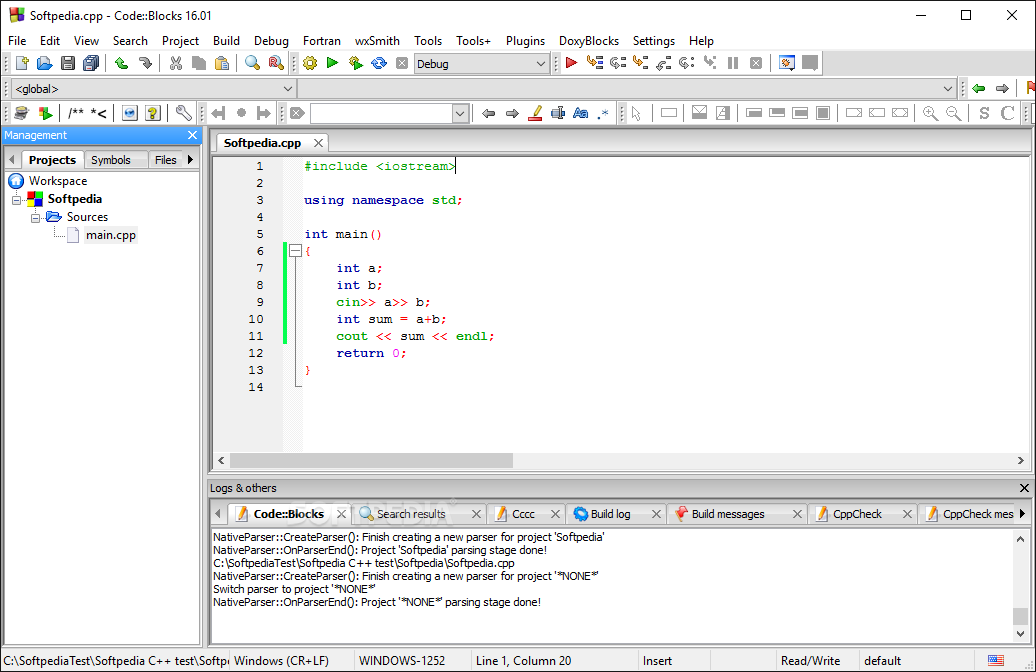
\includegraphics[width=0.5\paperwidth]{CodeBlocks}
\end{figure}

\subsection{Repl.it [Página web]}
Repl.it es una página web que te permite probar código desde cualquier plataforma, la unica desventaja puede ser que ocupes una cuenta para guardar tu código. Para usarlo, debe entrar a la página \url{https://repl.it/languages/cpp}

\begin{figure}[H]
    \centering
    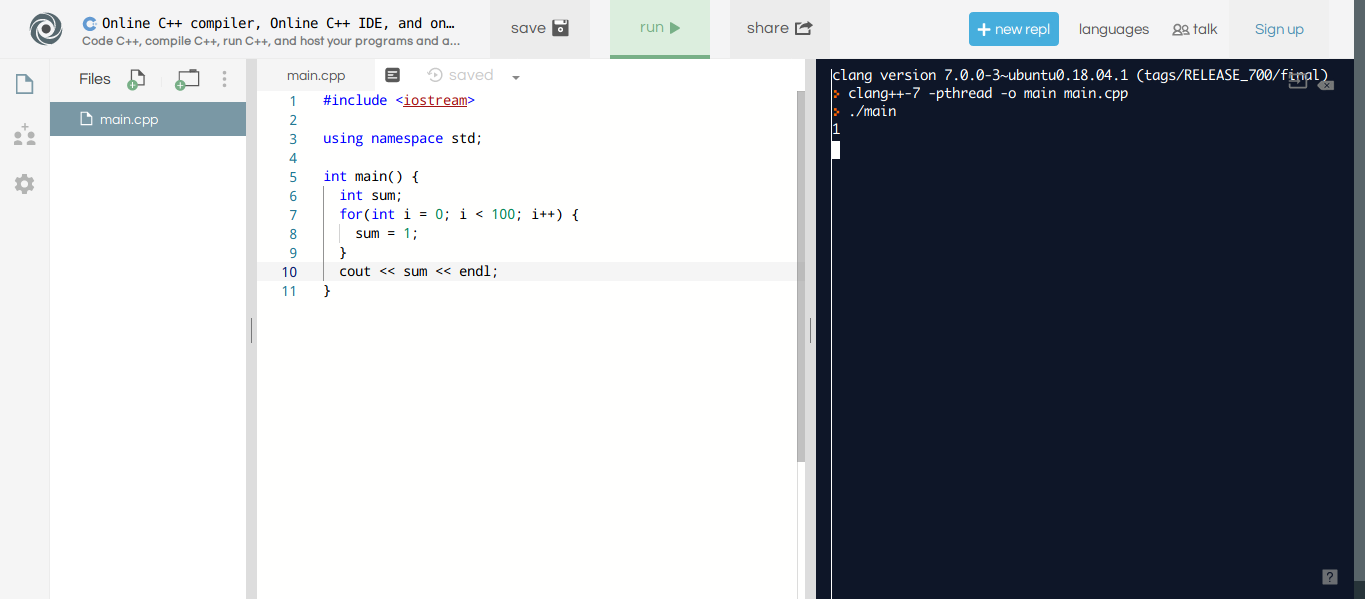
\includegraphics[width=0.5\paperwidth]{replit}
\end{figure}

\subsection{Visual Studio Community [Windows y Mac]}
Esta es la versión gratis del software famoso de Microsoft llamado Visual Studio, te permite compilar código en muchos lenguajes y ofrece herramientas avanzadas de analisis de código.

Se puede descargar en la página oficial \url{https://visualstudio.microsoft.com/vs/community/} y te permite usarlo siempre y cuando estes ingresado con una cuenta de Microsoft. Si no tienes una cuenta de Microsoft y quisiera utilizar este programa, puedes registrarte en \url{https://account.microsoft.com/account?lang=es-MX}

A pesar de que esta instalación es más tardado, es una opción bastante profesional y bueno si estas interesado en programar cosas más grandes.

\begin{figure}[H]
    \centering
    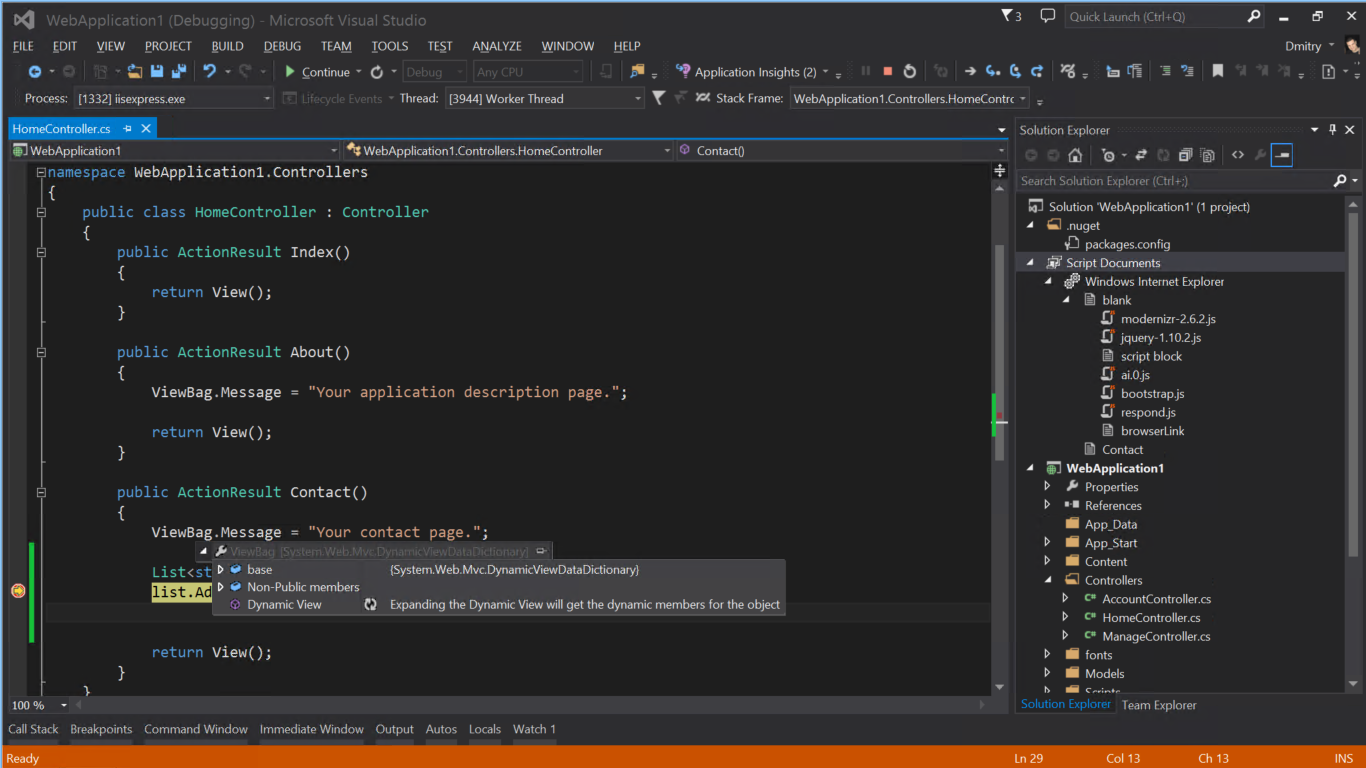
\includegraphics[width=0.5\paperwidth]{vscommunity}
\end{figure}

\subsection{Visual Studio Code + Terminal [Mac y Linux]}
El programa de Visual Studio Code es muy popular para la programación, tiene soporte para todos los lenguajes y es completamente gratis, con la desventaja de que no se puede compilar código.

Si estas en Windows, puedes utilizar este programa pero debes instalar algun emulador de terminal de sistemás Unix como mingw para compilar código.

Si estas usando Mac o Linux, puedes compilar un programa de C++ desde la terminal. Para hacer esto, debes asegurarte de tener instalado el paquete $gcc$ y debes generar un archivo ejecutable a partir del código con el comando $c++$

\begin{figure}[H]
    \centering
    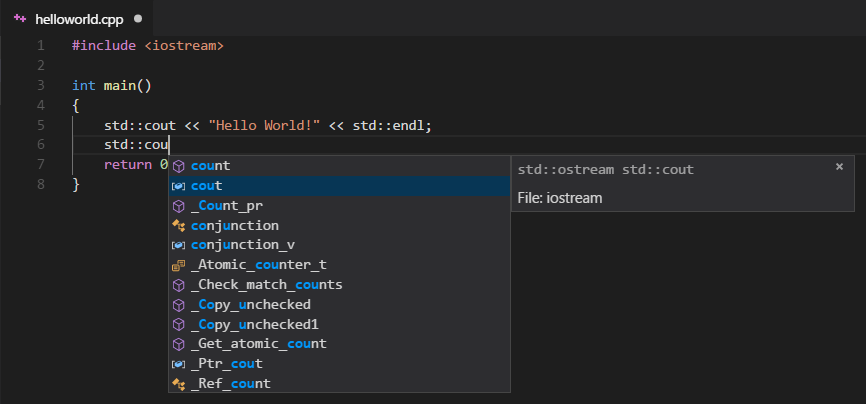
\includegraphics[width=0.5\paperwidth]{vscode}
\end{figure}

\section{¿Mi primer programa?}

\subsection{Donde empezar}

Antes de crear un programa, debes asegurarte que sabes lo que quieres que haga. Pero esto es algo muy dificil si vas empezando, ¡porque no tienes idea ni que puedes hacer con un programa!

Asi que durante estos proximos seis semanas, les daremos problemas de programación similares a los que aparecen en competencias más dificiles para que puedan aprender como crear sus propios programas para resolver problemas reales.

El programa más sencillo es uno que no hace nada; se abre y se cierra instantaneamente. Pero eso es aburrido y no tiene sentido. ¿Para qué quiero un programa que no hace nada?

Tu tienes que decirle al programa que quieras que haga, y el programa seguira tus instrucciones sin cuestionarlos, de tal grado que a veces cometera errores porque tu no esperabas que fuera a hacer todo al pie de la letra de como le dijiste.

Vamos a intentar construir un programa que sume dos números. Antes de empezar tu programa tendras que escribir cuatro lineas muy importantes. Si quitas alguno de estos cuatro lineas, tu programa dejara de funcionar y te arrojara un error, y ahorita es muy temprano para poder decirles exactamente lo que hacen estas lineas. Cuando tengan más experiencia, podrán cambiarlos a su gusto.

\begin{lstlisting}[language=C++, caption=Las cuatro lineas esenciales]
#include <iostream>

using namespace std;

int main() {

}
\end{lstlisting}

Ahí esta su primer programa, él que les dije que se abre y se cierra sin hacer nada. Por ahora, todo su código debe ir entre los dos corchetes.

Tenemos que decirle a nuestro programa que queremos dos números enteros, los cuales seran sumados después. Para cada número entero que queremos, tenemos que asignarle un nombre.

Para hacer esto, escribimos una linea para cada variable con int seguido por el nombre de la variable después (sin espacios y sin caracteres especiales). Finalmente, le ponemos un punto y coma después de cada linea para decirle que eso es lo unico que queremos hacer en esa linea.

\begin{lstlisting}[language=C++, caption=Dos variables]
#include <iostream>

using namespace std;

int main() {
    int a;
    int b;
}
\end{lstlisting}

Y asi tenemos dos números. Podemos nombrarlos como queramos, por ejemplo: numeroA y numeroB, alfa y beta, n1 y n2, etc. Si corremos el código, no pasa nada. Esto es porque no le hemos dicho al programa que queremos que haga con estos dos números, ni le hemos dicho que valores tienen.

En una linea, podemos escribir a = 5; para decirle que queremos que la variable a valga 5. Tambien es valido modificar la linea int b; para que sea int b = 2;

\begin{lstlisting}[language=C++, caption=Guardando valores]
#include <iostream>

using namespace std;

int main() {
    int a;
    a = 5;
    int b = 2;
}
\end{lstlisting}

Es de gran importancia saber que el programa lee el código desde arriba hacia abajo, asi que no podemos poner la linea que dice a = 5; antes de int a; porque no sabra que a es una variable que definimos.

Ahora solo falta decirle que queremos que sume a y b.

\begin{lstlisting}[language=C++, caption=Guardando valores]
#include <iostream>

using namespace std;

int main() {
    int a;
    a = 5;
    int b = 2;
    a + b;
}
\end{lstlisting}

Este nuevo programa parece sumarlos, pero si se corre tampoco pasa nada. Esto es porque tenemos que decirle al programa que además de sumarlos, queremos ver esta suma. Si no, calculará a + b, no sabrá que hacer con esa suma y lo descartará.

Para hacer que nos muestre este dato, tenemos que utilizar algo llamado cout, que no es nada mas que un comando que nos muestre datos.

Para usar cout, se debe escribir cout $<<$ valor; donde valor es lo que quieres ver.

\begin{lstlisting}[language=C++, caption=Tu primer programa]
#include <iostream>

using namespace std;

int main() {
    int a;
    a = 5;
    int b = 2;
    cout << a + b;
}
\end{lstlisting}
\href{https://repl.it/@Jamesscn/Mi-primer-programa}{Liga al código}\\

Y de esa manera, tenemos nuestro primer programa. Hay miles de maneras de hacer este mismo código, y todos son iguales de validos. Aqui mostraremos algunos ejemplos:

\begin{lstlisting}[language=C++, caption=¿El mismo programa?]
#include <iostream>

using namespace std;

int main() {
    int a = 5, b = 2;
    cout << a + b;
}
\end{lstlisting}

\begin{lstlisting}[language=C++, caption=¿El mismo programa?]
#include <iostream>

using namespace std;

int main() {
    int a;
    int b;
    int c;
    a = 5;
    b = 2;
    c = a + b;
    cout << c;
}
\end{lstlisting}

\begin{lstlisting}[language=C++, caption=¿El mismo programa?]
#include <iostream>

using namespace std;

int main() {
    cout << 2 + 5;
}
\end{lstlisting}

\subsection{Comentarios}

Una cosa muy util es que tu puedes escribir comentarios en medio de tu código y estos pueden servir para describir lo que hace cierto código, para recordarte de hacer algo en cierta parte o para mantener tu código ordenado.

El tipo de comentario mas popular es el de una sola linea, Estos se inician con dos $//$ seguidos por tu nota.

\begin{lstlisting}[language=C++, caption=Comentario]
#include <iostream>

using namespace std;

//Los comentarios pueden ir en lineas separadas
int main() {
    //En cualquier parte del codigo
    int a; //Incluso aqui!
    int b; 
    int c; //Esta variable es la suma de a y b
    a = 5;
    b = 2;
    c = a + b; //Aqui se hace la suma
    cout << c; //Aqui se imprime el resultado
}
\end{lstlisting}

Tambien existen los comentarios de multiples lineas, estos se deben iniciar con $/*$ y se deben terminar con $*/$

\begin{lstlisting}[language=C++, caption=Comentario]
#include <iostream>

using namespace std;

/*  Esto es un comentario de multiples lineas
    Puedes escribir cuantas lineas quieras aqui
    Tambien sirve para temporalmente deshabilitar codigo
*/
int main() {
    int a; /* Tambien debes saber que pueden ocupar una sola linea */
    int b; 
    int c;
    a = 5;
    b = 2;
    c = a + b;
    cout << c;
}
\end{lstlisting}

\section{Leyendo y escribiendo}

A la hora de compilar y ejecutar tu programa, seguramente notaste que se abre una consola con todo lo que decidiste ver. Esto es porque C++ corre dentro de esa consola (Tu compilador ejecuta comandos para abrir el programa sin que tu veas).

Esto te permite leer y escribir datos mientras que tu programa corre. Ya se ha visto que para escribir datos, se puede utilizar cout (que significa c + out o output de C) seguido por la variable que quieres "imprimir" a la consola.

Para leer datos, se ocupa tener una variable para almacenar ese dato de entrada, luego se debe utilizar cin (que significa c + in o input de C) seguido por esa variable.

Estas dos herramientas te permiten crear programas generales que resuelven problemas especificos.

Digamos que queremos crear un programa que lee dos números enteros (sin importar cuales sean) y que imprime su suma. Podemos crear este programa utilizando cin y cout para que el usuario diga cuales dos números quiere que sume.

\begin{lstlisting}[language=C++, caption=Suma]
#include <iostream>

using namespace std;

int main() {
    int a, b;
    cin >> a >> b;
    cout << a + b << endl;
}
\end{lstlisting}
\href{https://repl.it/@Jamesscn/Suma}{Liga al código}\\

Cuando ejecutas tu código, veras que la consola esta esperando una entrada. Puedes ingresar dos numeros separados por espacios y picarle enter o poner el primer numero, picar enter, poner el segundo y picarle enter denuevo. Al terminar de hacer eso, veras que tu programa hace la suma instantaneamente y que lo despliega debajo de los numeros que le diste.

\section{Errores comunes}

\subsection{Falta de inicialización}
Este error es uno de los más graves y más dificiles de detectar debido a que la lógica puede estar completamente correcta, el programa se compila sin errores y en algunos casos tus variables te podran dar los resultados correctos.

Esto pasa cuando defines una variable pero no le das un valor inicial. Por ejemplo:

\begin{lstlisting}[language=C++, caption=Error de inicialización]
#include <iostream>

using namespace std;

int main() {
    int i = 1;
    int suma;
    while(i <= 100) {
        suma += i;
        i++;
    }
    cout << suma << endl;
}
\end{lstlisting}
\href{https://repl.it/@Jamesscn/Suma-Imposible}{Liga al código}\\

Este programa suma los números de 1 a 100 y los va guardando en la variable suma. Se esperaría que el resultado fuera 5050, pero si lo corres te despliega -1428474. Si vuelves a correr el código, ahora ves 82934. Este valor siempre cambia.

Esto ocurre debido a que nunca inicializamos o le damos un valor inicial a la variable suma. A la hora de declarar la variable, le estamos asegurando un espacio en la memoria del sistema pero esto no significa que ese espacio tenga guardado un cero. Puede ser que algun proceso anterior haya tenido que usar ese espacio y que haya dejado un valor que no nos interesa ahí.

La razón por la que siempre cambia es porque la memoria siempre esta siendo utilizado por otros procesos (Google Chrome, Word, etc.) y cada vez que corre el programa agarrara el primer espacio libre que encuentra para la variable suma, que no siempre será la misma.

Existe una posibilidad de que tu compilador automaticamente detecte que suma no fue inicializado y le asigna el valor de cero después, esto puede provocar que el programa funcione en tu computadora pero a la hora de probarlo en otra falla.

Entonces para asegurar que esto nunca pase, siempre debes de tener la costumbre de inicializar tus variables a menos que sabes que serán sobreescritos por otro valor o leidos desde la consola usando $cin$.

\subsection{Ciclos con otras variables}
Este error pasa muy seguido cuando se utilizan ciclos for anidados y cuando uno olvida que haya declarado una variable antes.

Digamos que vas tan mal en matemáticas que se te olvidaron las tablas multiplicativas por completo, y tu quieres crear un programa que los genera. Puedes hacer esto con dos ciclos for anidados, uno que calcule las filas y otra que calcule las columnas.

\begin{lstlisting}[language=C++, caption=Ciclos con otras variables]
#include <iostream>

using namespace std;

int main() {
    for(int i = 0; i <= 12; i++) {
        for(int j = 0; i <= 12; i++) {
            cout << i * j << "\t";
        }
        cout << endl;
    }
}
\end{lstlisting}
\href{https://repl.it/@Jamesscn/Tablas-de-Falsedad}{Liga al código}\\

Al parecer este código esta bien, pero si miras fijamente verás que en el segundo ciclo estamos modificando i en lugar de j. El compilador asume que sabes lo que estas haciendo, asi que no te arrojá ningun error al tener distintos variables en un solo ciclo.

Para asegurar que esto no pase, siempre debes asegurarte de que solo estes modificando una variable por ciclo y que no hayas usado una variable con ese mismo nombre antes.

\subsection{Error por uno}
Este error tiende a ser muy facil de arreglar y ocurre por fallas de lógica.

Digamos que quieres encontrar la suma de todos los cuadrados $1^2 + 2^2 + 3^2 ... + n^2$, y creas un programa para calcularlo.

\begin{lstlisting}[language=C++, caption=Error por uno]
#include <iostream>

using namespace std;

int main() {
    int n;
    cin >> n;
    int suma = 0;
    for(int i = 0; i < n; i++) {
        suma += i * i;
    }
    cout << suma << endl;
}
\end{lstlisting}
\href{https://repl.it/@Jamesscn/Sumás-Cuadrados}{Liga al código}\\

Corres tu programa con $n = 3$, y ya sabes que $1^2 + 2^2 + 3^2 = 1 + 4 + 9 = 14$, pero te dice que es 5. Ahora corres tu programa con $n = 4$ y ahora observas que la respuesta es 14 cuando debía ser 30. Esto ocurre porque estas contando de $0$ a $n-1$ (nota que el for tiene la expresión i < n cuando debía ser i <= n).

Esto pasó porque el for loop cuenta hasta n pero no lo incluye en la suma, y estos tipos de errores suelen ocurrir cuando se utilizan ciclos que inician desde 1 o cuando se debe incluir el ultimo valor en el proceso.

\subsection{Segmentation fault}
Este error es algo común y suele pasar cuando quieres sacar un valor que esta fuera de un arreglo.

Digamos que tenemos un código que le pregunta al usuario un valor y luego despliega el factorial de ese valor. El código asume que el usuario seleccionará un número entre 0 y 10, para luego desplegar su factorial el cual esta guardado en un arreglo.

\begin{lstlisting}[language=C++, caption=Error de inicialización]
#include <iostream>

using namespace std;

int main() {
    int factoriales[] = {1, 1, 2, 6, 24, 120, 720, 5040, 40320, 362880, 3628800};
    cout << "Que factorial quisieras?" << endl;
    int deseado;
    cin >> deseado;
    if(deseado < 0) {
        cout << "No existe " << deseado << "!";
    } else {
        cout << deseado << "! es " << factoriales[deseado] << endl;
    }
}
\end{lstlisting}
\href{https://repl.it/@Jamesscn/Indices-Inexistentes}{Liga al código}\\

Ahora que pasa si el usuario quiere saber el valor de 25565 factorial? Si ejecutas el código con tal valor verás que el programa se cierra inesperadamente y regresa el siguiente error: [1] 12937 segmentation fault (core dumped).

Esto ocurre porque estas intentando accesar el elemento 25565 de un arreglo que solo tiene 10 valores, lo que pasa es que estas intentando ver un lugar que no existe en la memoria de tu programa.

El 95\% de las veces que verás un segmentation fault, será porque estas intentando modificar o ver un valor que esta fuera de un arreglo. Siempre debes asegurarte que un arreglo tiene suficiente espacio para guardar todos los posibles valores que ocupes.

\subsection{Sobreflujos}
Este error pasa cuando tienes un valor que es demásiado grande para una variable.

Ahora vamos a mejorar el código que habiamos hecho del factorial. En lugar de guardar los primeros 10 valores en un arreglo, vamos a generar cada valor con un ciclo.

Para checar que todo este bien, voy a desplegar los primeros 18 factoriales.

\begin{lstlisting}[language=C++, caption=Sobreflujo]
#include <iostream>

using namespace std;

int main() {
    int factorial = 1;
    for(int i = 1; i < 18; i++) {
        factorial *= i;
        cout << factorial << endl;
    }
}
\end{lstlisting}
\href{https://repl.it/@Jamesscn/Sobrefactorial}{Liga al código}\\

Corres este código y te topas con una sorpresa, 17! es aparentemente -288522240. ¿Cómo fue que un factorial te dio un número negativo si siempre incrementa?

Lo que esta pasando es que el valor de 17! es demásiado grande para ser guardado en un valor de tipo int, si buscas en linea encontraras que un int solo puede guardar valores de -2,147,483,648 a 2,147,483,647, y 17! tiene un valor de 355,687,428,096,000.

El programa no te arroja ningun error, simplemente lo que hace es que cuando un número es más grande del valor máximo de 2,147,483,647, se traslapa a -2,147,483,648 y sigue sumando desde ese valor. Eso significa que si quiero guardo el valor de 2,147,483,649 en un int, me guardará en realidad el valor -2,147,483,647.

Si sigues imprimiendo más números, verás que se vuelven a hacer positivos y negativos debido a este traslape.

Para solucionar esto, debes reemplazar int por otro tipo de dato que pueda guardar números más grandes, como long long int o double.

\subsection{Errores de redondeo}
Este error pasa cuando se dividen dos enteros.

Sabes que $\frac{1}{2} + \frac{1}{4} + \frac{1}{8} + \frac{1}{16} + ... = 1$ y quisieras comprobarlo creando un programa. Lo implementas con el siguiente código:

\begin{lstlisting}[language=C++, caption=Error de redondeo]
#include <iostream>

using namespace std;

int main() {
    int suma = 0;
    int potencia = 2;
    for(int i = 1; i < 30; i++) {
        suma += 1 / potencia;
        potencia *= 2;
    }
    cout << suma << endl;
}
\end{lstlisting}
\href{https://repl.it/@Jamesscn/Suma-Fraccional}{Liga al código}\\

Pero cuando lo corres, te dice que tu suma es cero. Revisas la variable de potencia y te das cuenta que ese sí esta bien, pero la variable de suma se queda en cero.

Esto ocurre debido a que 1 y potencia estan siendo guardados como enteros, y cuando se dividen dos enteros el resultado siempre será otro entero redondeado para abajo. Es decir si hago $5 / 2$, esto me dará $2$ porque el valor de $2.5$ fue redondeado hacia abajo. Como potencia siempre es mayor que 1, esta division siempre se redondeara para abajo y dará cero.

Para corregir esto, se deben cambiar las variables de potencia y de suma de enteros a un tipo de dato flotante, es decir un número que permite puntos decimales.

\subsection{Faltas de memoria}
Esto sucede cuando tu programa ocupa demásiado espacio continuo y ocasiona un error.

A veces sucede que tienes que crear un arreglo con 10 millones de valores (es verdad, sí vas a ocupar algo asi!) y te darás cuenta que tu programa deja de funcionar.

\begin{lstlisting}[language=C++, caption=Faltas de memoria]
#include <iostream>

using namespace std;

int main() {
    int arreglo[10000000];
    for(int i = 0; i < 10000000; i++) {
        arreglo[i] = i;
    }
    cout << "Arreglo llenado" << endl;
}
\end{lstlisting}
\href{https://repl.it/@Jamesscn/Arreglo-no-arreglado}{Liga al código}\\

Por suerte, esto se puede arreglar. Si cuentas los bytes, te darás cuenta que son 4 millones de bytes o 4 megabytes, y las computadoras modernas tienden a tener hasta 16 gigabytes de memoria RAM, asi que no debe haber problema para conseguir 4 megabytes de memoria.

El problema viene del hecho que a la hora de crear un arreglo, el sistema busca 4 megabytes de espacio que estén libres y juntos dentro de la memoria del programa. Esto se puede arreglar preguntandole a tu sistema si puedes guardar estos 4 megabytes en una area especial extra de memoria llamado el heap, que viene siendo una area publica con muchisimo espacio, en lugar del espacio limitado que fue asignado a tu programa.

Para hacer que el programa busque dentro del heap, debes cambiar el arreglo a un puntero y utilizar malloc, new o alguna funcion que te permite obtener espacio del heap.

\section{Tipos de datos}

\subsection{Signed y unsigned}

\subsection{Numericos}

\subsection{Caracteres y cadenas}

\subsection{Booleanos}

\subsection{Long long}

\subsection{Arreglos}

\section{Funciones}

Las funciones son muy utiles para cuando tienes que repitir código similar muchas veces. Estos son similares a funciones matemáticas, reciben cuantas variables de entrada quieres que tengan, haran una operación con estas entradas y regresará una sola variable de salida.

Para una función, se dice que se "regresa" su salida porque para indicar que se quiere terminar la función, se utiliza el operador $return$ seguido por el valor de la variable de salida.

Un ejemplo sencillo es una función que suma dos números enteros A y B y que regresa otro entero C, la suma. Esto lo podemos implementar de la siguiente manera:

\begin{lstlisting}[language=C++, caption=Función de suma]
    int suma(int a, int b) {
        int c = a + b;
        return c;
    }
\end{lstlisting}

Como se puede ver, se inicia una funcion con un tipo de dato que corresponde a el tipo de dato de la salida. Como int va antes que el nombre de la función (suma), nos dice que queremos que regrese un entero.

Luego, sigue el nombre de la función y dos parentesis. Dentro de los parentesis van las variables de entrada separadas por comas. Como tenemos un entero a y otro entero b, estamos diciendo que para correr esta función el usuario debe dar dos números en ese orden, los cuales serán guardados en a y b.

Luego, siguen corchetes que encapsulan el código de la función. Aqui es donde hacemos nuestros cálculos con nuestras variables y regresamos el valor de la salida.

Declaramos otro entero c y le asignamos la suma de a y b, luego lo regresamos, es decir estamos diciendo que queremos que c sea nuestra salida.

Todas las funciones tienen que estar colocados antes de main de tal manera:

\begin{lstlisting}[language=C++, caption=Función de suma]
    #include <iostream>

    using namespace std;
    
    int suma(int a, int b) {
        int c = a + b;
        return c;
    }

    int main() {

    }
\end{lstlisting}

Ahora, podemos llamar nuestra función dentro de main dandole los parametros que queremos:

\begin{lstlisting}[language=C++, caption=Función de suma]
    #include <iostream>

    using namespace std;
    
    int suma(int a, int b) {
        int c = a + b;
        return c;
    }

    int main() {
        cout << suma(3, 5) << endl;
    }
\end{lstlisting}
\href{https://repl.it/@Jamesscn/Funciones}{Liga al código}\\

Al ejecutar este código, nos despliegara un 8.

Otro ejemplo es una función que regresa la división de dos enteros:

\begin{lstlisting}[language=C++, caption=Función de división]
    #include <iostream>

    using namespace std;
    
    float divide(int a, int b) {
        return (float)a / b;
    }

    int main() {
        cout << divide(5, 2) << endl;
    }
\end{lstlisting}
\href{https://repl.it/@Jamesscn/Funciones}{Liga al código}\\

Este código imprime 2.5, lo que hace es que recibe dos enteros a y b, y luego regresa su división como si fuera un número flotante. El (float) antes del a significa que quieres convertir la división en un número flotante antes de que redondea.

\end{document}

